\documentclass{beamer}

\usepackage{Vor2018glærur}

\title{Tölvunarfræði 2}
\subtitle{Vika 4}

\begin{document}

\begin{frame}
	\titlepage
\end{frame}

\section{Inngangur}

\begin{frame}{Spurningar úr síðasta tíma}
	\begin{itemize}
		\item Er hægt að athuga tag klasa í C++?
		      \begin{itemize}
			      \item Já, sjá \href{https://docs.microsoft.com/en-us/cpp/cpp/typeid-operator}{typeid}
		      \end{itemize}
		\item Hver er sjálfgefna aðgangsstýringin í C++?
		      \begin{itemize}
			      \item Það er \texttt{private}. Sjá \href{https://raw.githubusercontent.com/Ernir/kennsluefni/master/T2/Code/w2/singlylinked.cpp}{singlylinked.cpp} úr viku 2, það þýðist ekki sé ``public'' lykilorðið fjarlægt
			      \item Sjálfgefið er að \texttt{struct} í C-stíl hafi \texttt{public} aðgangsstýringu
		      \end{itemize}
	\end{itemize}
\end{frame}

\begin{frame}{Skoðanakönnun}

	Athygli er vakin á \href{https://piazza.com/class/jc3kcn5f4sn1cc?cid=95}{ráðgefandi skoðanakönnun} um mögulega tilfærslu á verkefnaskiladeginum.
	
\end{frame}

\begin{frame}{Af hverju er T2 svona erfið?}
	\begin{itemize}
		\item Við erum að fást við önnur vandamál en í Tölvunarfræði 1
		\item Gömul\footnote{\emph{Some Difficulties of Learning to Program}, du Boulay, 1986} flokkun á ``erfiðleikunum við að forrita''
		      \begin{itemize}
			      \item Orientation - til hvers er forritun og hverju er hægt að ná fram?
			      \item Notation - málfræði og merking ákveðins forritunarmáls
			      \item The machine - þekking á tölvunni sem forritunartóli
			      \item Structures - ``þekktar lausnir'' sem hægt er að nota aftur
			      \item Pragmatics - almennir hæfileikar við skipulagningu, aflúsun, prófanir o.fl.
		      \end{itemize}
		\item Tölvunarfræði 1 tók að miklu leyti á fyrstu tveimur atriðunum
		\item Tölvunarfræði 2 hamrar á fjórða atriðinu
		      \begin{itemize}
			      \item Forritunargrunnur er nauðsynlegur en ekki nægjanlegur \pause
			      \item En þetta venst
		      \end{itemize}
	\end{itemize}
\end{frame}

\section{Java og hlutbundin forritun}

\begin{frame}{Java}
	\begin{columns}
		\column{0.6\textwidth}
		\begin{itemize}
			\item Munum héðan af líka forrita í Java, auk C++
			\item Þekkjum það vonandi flest úr Tölvunarfræði 1!
			      \begin{itemize}
				      \item Ef ekki - setja upp Java-þýðanda (\texttt{javac}) sem allra fyrst, ásamt forritssafni bókahöfunda (\texttt{algs4.jar})
				      \item Leiðbeiningar á \href{http://algs4.cs.princeton.edu/code/}{síðu bókarinnar}
			      \end{itemize}
			\item Java líkist C++ að ýmsu leyti
		\end{itemize}
		\column{0.4\textwidth}
		\begin{center}
			
\includegraphics[width=\textwidth]{java}
		\end{center}
	\end{columns}
\end{frame}

\begin{frame}{Lykilorðið \texttt{static}}
	\begin{itemize}
		\item Í Java tilheyra allar aðferðir klösum, líka \texttt{main} aðferðir
		\item Þurfum að ákvarða hvort að aðferðir sem við búum til tilheyri \emph{klasa} eða \emph{tilviki af klasa}
		      \begin{itemize}
			      \item Tilviksaðferðir \texttt{instance methods} tilheyra tilviki, er sjálfgefið
			      \item Klasaaðferðir \eng{class methods} tilheyra klasa
		      \end{itemize}
		\item Tilsvarandi á við um eiginleika klasa \eng{class properties}
		\item Dæmi um klasa með mörgum klasaaðferðum: \href{https://docs.oracle.com/javase/8/docs/api/java/lang/Math.html}{\texttt{Math}}
	\end{itemize}
\end{frame}

\begin{frame}{Dæmi}
	\javafile[firstline=3, lastline=21, fontsize=\scriptsize, label=StaticExample.java]{Code/w4/StaticExample.java}
\end{frame}

\begin{frame}[fragile]{Mismunandi gagnagerðir}
	\begin{itemize}
		\item Í Java höfum við tvær tegundir af gagnagerðum
		      \begin{itemize}
			      \item Einfaldar gerðir \eng{primitive types}, örfáar innbyggðar
			      \item Tilvísunargerðir \eng{reference types}, allt sem skilgreint er af klösum
		      \end{itemize}
		\item Dæmi: \texttt{int} er einföld gerð fyrir heiltölur, \texttt{Integer} er tilvísunargerð
	\end{itemize}
\end{frame}

\begin{frame}[fragile]{Að smíða tilvik}
	Þegar Java forrit notar \texttt{new} er minnissvæði í kös frátekið, kallað á smið og tilvísun (e. \emph{reference}) á hlutinn skilað
	\begin{center}
		Tilvik af klasanum \texttt{A} búið til:

		\vspace{-0.5cm}
	\end{center}
	\begin{columns}
		\column{0.5\textwidth}
		\begin{minted}[frame=lines, label=Java]{java}
A a = new A();
\end{minted}
		\column{0.5\textwidth}
		\begin{minted}[frame=lines, label=C++]{cpp}
A *a = new A();
\end{minted}
	\end{columns}
\end{frame}

\begin{frame}{Dæmi}
	Lítum á \texttt{ObjectInstantiation.java}.
\end{frame}

\begin{frame}{Erfðir og Object}
	\begin{itemize}
		\item \emph{Allir} klasar í Java erfa frá innbyggða klasanum \texttt{Object}
		\item Þurfum ekki að taka erfðirnar fram
		      \begin{itemize}
			      \item \href{https://docs.oracle.com/javase/8/docs/api/java/lang/Object.html}{Object} á síðu Oracle
		      \end{itemize}
		\item Þetta þýðir að tilvik af öllum klösum í Java hafa nokkrar aðferðir sem skipta okkur máli:
		      \begin{itemize}
			      \item \texttt{toString}
			      \item \texttt{equals}
			      \item \texttt{hashCode} (sjáum meira um seinna)
		      \end{itemize}
	\end{itemize}
\end{frame}

\begin{frame}{Jafngildi hluta}
	\begin{itemize}
		\item Sjáum að jafngildi er skilgreint með \texttt{equals} aðferð
		      \begin{itemize}
			      \item \texttt{equals} aðferð á að vera jafngildisvensl \eng{equivalence relation}
			            \begin{itemize}
				            \item Sjálfhverft \eng{reflexive}: \texttt{x.equals(x)} skal vera satt
				            \item Samhverft \eng{symmetric}: \texttt{x.equals(y)} þá og því aðeins að \texttt{y.equals(x)}
				            \item Gegnvirk \eng{transitive}: Ef \texttt{x.equals(y)} og \texttt{y.equals(z)} þá skal \texttt{x.equals(z)}
			            \end{itemize}
			      \item Einnig skal \texttt{x.equals(y)} alltaf skila sama gildi og \texttt{x.equals(null)} alltaf skila ósönnu
		      \end{itemize}
		\item Okkar klasar gætu þurft að útfæra \texttt{equals} aðferð
	\end{itemize}
\end{frame}


\begin{frame}[fragile]{Gildisveiting breyta}
	Gildra: Gildisveiting afritar gildi á einföldum breytum, en afritar vísun á breytu af tilvísunargerð!

	\javafile[firstline=34, lastline=39, fontsize=\scriptsize, gobble=8, label=IntegerBox.java]{Code/w4/IntegerBox.java}
\end{frame}

\begin{frame}{Breytur og aðferðir}
	Gildra: Þegar aðferðir taka við breytum, þá eru breyturnar afritaðar. Þegar breytan er einföld er gildi hennar afritað, en sé hún af tilvísunargerð er vísunin í hana afrituð.

	\javafile[firstline=8, lastline=17, gobble=4, fontsize=\scriptsize, label=PassingVariables.java]{Code/w4/PassingVariables.java}
\end{frame}

\section{Fjölnota klasar}

\begin{frame}{Dæmi}
	\begin{columns}
		\column{0.55\textwidth}
		\begin{itemize}
			\item Hingað til hefur verið ákveðin takmörkun á reikniritum og aðferðum - þær virka bara á eina gagnagerð
			\item Við getum útvíkkað klasana okkar og aðferðir með því að skilgreina þau sem fjölnota (e. \emph{generic})
		\end{itemize}
		\column{0.45\textwidth}
		\begin{center}
			\javafile[fontsize=\scriptsize, firstline=3, lastline=12,label=Genericbox.java]{Code/w4/GenericBox.java}

			Kassi fyrir alls kyns hluti.
		\end{center}
	\end{columns}
\end{frame}

\section{Almennar forritslýsingar}

\begin{frame}{Skil (APIs)}
	\begin{itemize}
		\item Til að auðvelda samskipti forrita skilgreinum við oft fyrir þau skil (e. \emph{Application Programming Interfaces}, APIs)
		\item Í skilum felast notkunar- og samskiptalýsingar á aðferðum og sviðum
		\begin{itemize}
			\item Vel skilgreindur API hjálpar okkur að nota forrit annarra og hjálpar öðrum að nota okkar forrit
		\end{itemize}
		\item Skil eru sérstaklega mikilvæg fyrir forritasöfn \eng{libraries}
		\item Hugmyndin - ef við vitum hvernig hitt forritið hegðar sér þarf forritið okkar ekki að hafa aðgang að útfærslu þess
		\item Felur í sér n.k. samning á milli forrita
	\end{itemize}
\end{frame}

\begin{frame}{Dæmi}
	\begin{center}
		Skil fyrir teljara. Algorithms, bls. 65.

		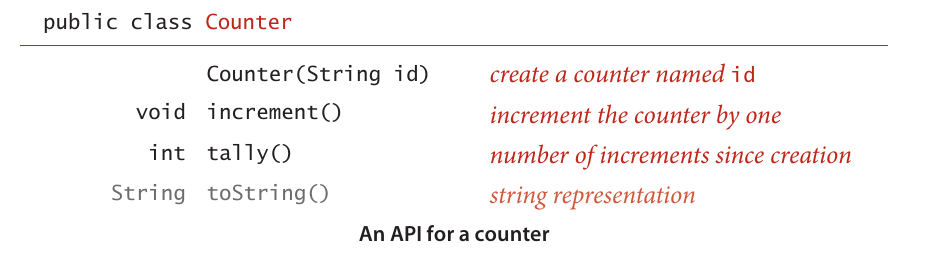
\includegraphics[width=\textwidth]{counter-api}
	\end{center}
\end{frame}

\begin{frame}[fragile]{Skil (interfaces)}
	\begin{itemize}
		\item Java hefur innbyggðan stuðning fyrir skil \eng{interfaces}
		      \begin{itemize}
			      \item Íslenska orðið ``skil'' virðist vera notað yfir bæði APIs og interfaces
		      \end{itemize}
		\item Í interface felst ``loforð'' um að klasi útfæri ákveðna virkni
		\item Getum sagt að klasi \texttt{A} eigi að útfæra skil \texttt{B} með
		      \begin{minted}{java}
class A implements B
	\end{minted}
		\item Þegar klasi útfærir interface þarf hann að innihalda útfærslu á öllum aðferðum sem lýst er í interface-inu
		\item Interfaces sem við munum sjá meira af:
		      \begin{itemize}
			      \item \href{https://docs.oracle.com/javase/8/docs/api/java/lang/Comparable.html}{Comparable}, \href{https://docs.oracle.com/javase/8/docs/api/java/lang/Iterable.html}{Iterable} og \href{https://docs.oracle.com/javase/8/docs/api/java/util/List.html}{List}
		      \end{itemize}
	\end{itemize}
\end{frame}

\begin{frame}{Hugrænar gagnagerðir}
	\begin{itemize}
		\item Hugræn gagnagerð (e. \emph{Abstract Data Type, ADT}) er gagnagerð þar sem útfærslan er falin fyrir þeim sem nota gagnagerðina
		\item Getum útbúið skil (API) til að skilgreina hugræna gagnagerð
		      \begin{itemize}
			      \item Þegar við \emph{notum} hugræna gagnagerð beitum við aðferðunum sem skil hennar skilgreina
			      \item Þegar við \emph{útfærum} hugræna gagnagerð einbeitum við okkur að uppröðun gagnanna og gætum þess að skilin séu uppfyllt
		      \end{itemize}
		\item Dæmi um hugrænar gagnagerðir: skjóður, hlaðar og biðraðir
		\item Ath: Eintengdur listi er ekki \emph{hugræn} gagnagerð, heldur bara gagnagerð \eng{data structure}
	\end{itemize}
\end{frame}
\section{Lokaorð}

\begin{frame}{Þessi glærupakki}
	Öll nafngreind forrit í þessum glærupakka, ásamt glærupakkanum sjálfum, má finna á  \href{https://github.com/Ernir/kennsluefni/tree/master/T2/Code/w4}{Github}.

	Fleiri forrit: \url{http://algs4.cs.princeton.edu/code/}
\end{frame}


\begin{frame}{Næst}
	Skjóður, biðraðir, hlaðar, greining reiknirita
\end{frame}


\end{document}
